%Copyright 2014 Jean-Philippe Eisenbarth
%This program is free software: you can 
%redistribute it and/or modify it under the terms of the GNU General Public 
%License as published by the Free Software Foundation, either version 3 of the 
%License, or (at your option) any later version.
%This program is distributed in the hope that it will be useful,but WITHOUT ANY 
%WARRANTY; without even the implied warranty of MERCHANTABILITY or FITNESS FOR A 
%PARTICULAR PURPOSE. See the GNU General Public License for more details.
%You should have received a copy of the GNU General Public License along with 
%this program.  If not, see <http://www.gnu.org/licenses/>.

%Based on the code of Yiannis Lazarides
%http://tex.stackexchange.com/questions/42602/software-requirements-specification-with-latex
%http://tex.stackexchange.com/users/963/yiannis-lazarides
%Also based on the template of Karl E. Wiegers
%http://www.se.rit.edu/~emad/teaching/slides/srs_template_sep14.pdf
%http://karlwiegers.com


\documentclass{scrreprt}

\usepackage{pdfpages}
\usepackage{listings}
\usepackage[T1]{fontenc}
\usepackage{placeins}
\usepackage{float}
\usepackage{underscore}
\usepackage[bookmarks=true]{hyperref}
\usepackage[utf8]{inputenc}
\usepackage{graphicx}
\usepackage{subfigure}
\usepackage{xcolor,listings}
\usepackage[english]{babel}
\hypersetup{
	bookmarks=false,    % show bookmarks bar?
	pdftitle={Data Mining},    % title
	pdfauthor={Adam-Ryan},                     % author
	pdfsubject={TeX and LaTeX},                        % subject of the document
	pdfkeywords={TeX, LaTeX, graphics, images}, % list of keywords
	colorlinks=true,       % false: boxed links; true: colored links
	linkcolor=blue,       % color of internal links
	citecolor=black,       % color of links to bibliography
	filecolor=black,        % color of file links
	urlcolor=blue,        % color of external links
	linktoc=page            % only page is linked
}%
\def\myversion{1.0}
\date{}
%\title
\usepackage{hyperref}
\begin{document}
	
	\begin{flushright}
		\rule{16cm}{5pt}\vskip1cm
		\begin{bfseries}
			\Huge{Tutorial 5\\}
			\vspace{1.9cm}
			for\\
			\vspace{1.9cm}
			Data Mining - Simple Modelling
			\vspace{1.9cm}
			\LARGE{Version \myversion}\\
			\vspace{1.9cm}
			Adam Ryan (14395076)\\
			\vspace{1.9cm}
			COMP47530\\
			\vspace{1.9cm}
			\today\\
		\end{bfseries}
	\end{flushright}
	
	\tableofcontents

	
\chapter{Question 1}
\section{Questions and answers}\label{E1Q}
The file ./specs/marks\_question1.csv contains data about midterm and final exam grades for a group of students.

\begin{enumerate}
	\item  Plot the data using matplotlib. Do midterm and final exam seem to have a linear relationship? Discuss the data and their relationship in your report. Save your plot to ./output/marks.png.
	\begin{itemize}
		\item We see that midterm and final appear to exhibit a linear relationship, with final increasing as midterm increases. We see there's a strong correlation of 0.78 between the two variables. We see that we've twelve records in each with the data skewed towards higher marks. The key summary stats are shown in figure \ref{stats} while the correlation matrix is shown in figure \ref{corr} and the seemingly linear relationship between the variables in figure \ref{q1a}.
		\begin{figure}[h!]
		\centering
		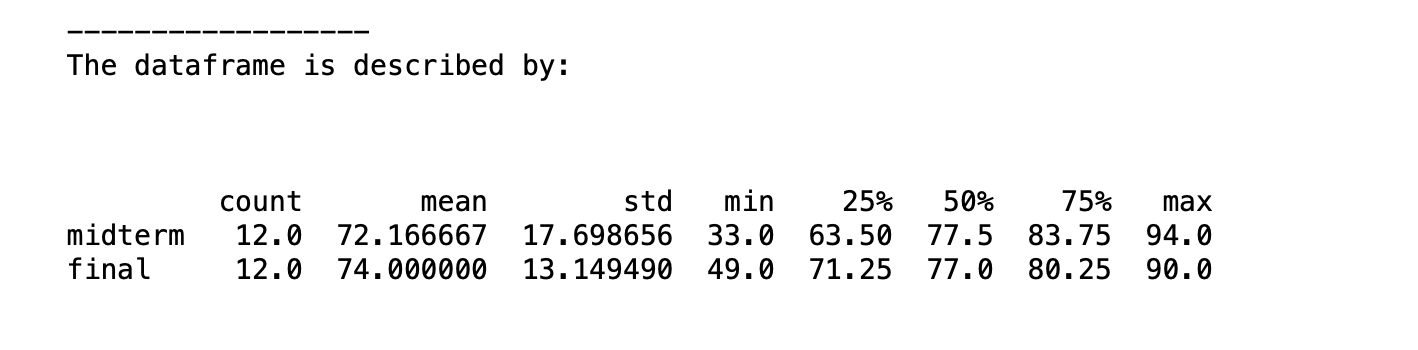
\includegraphics[width=0.7\linewidth]{exam_desc.png}
		\caption{Dataframe Summary Statistics}\label{stats}
		\end{figure}
	
		\begin{figure}[h!]
			\centering
			\includegraphics[width=0.5\linewidth]{exam_correlation_heatmap.png}
			\caption{Correlation Matrix for Exam}\label{corr}
		\end{figure}
			
			\begin{figure}[h!]
				\centering
				\includegraphics[width=0.5\linewidth]{marks.png}
				\caption{Midterm vs Final}\label{q1a}
			\end{figure}
	
	\end{itemize}

\pagebreak
	\item Use linear regression to generate a model for the prediction of a students’ final exam grade based on the students’ midterm grade in the course, then describe the model in your report.
	\begin{enumerate}
		\item I have generated a model using SKLearn. The model is:\\
		$final(midterm) = 
		(midterm * 0.5816000773918931) + (32.02786108155171)$
		\item This model has an RMSE of 7.8 and an $r^2$ of 0.61. Over 5-folds, the average RMSE is 8.6 with a standard deviatio of the RMSE of 3.3.
		\item Ultimately the volume of data we have is pretty low. 
		\item As per the lecture notes I've trained the model on the entire data set.
		\item The model can be visualised as in \ref{data} and \ref{q1c}:
		
				\begin{figure}[h!]
			\centering
			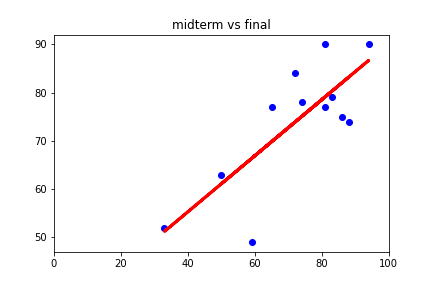
\includegraphics[width=0.5\linewidth]{Data with Regression.png}
			\caption{Regression Line on Data}\label{data}
		\end{figure}
		
		\begin{figure}[h!]
			\centering
			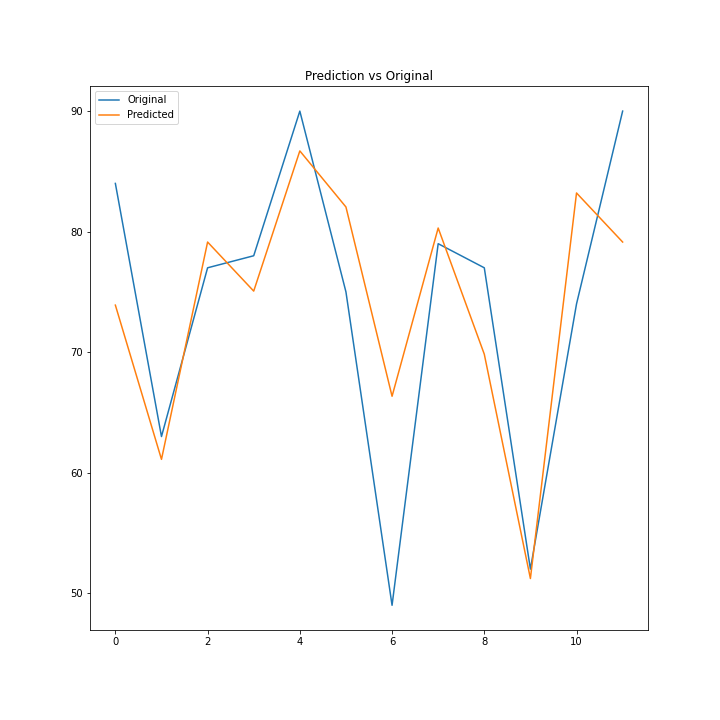
\includegraphics[width=0.5\linewidth]{linear_prediction_vs_original.png}
			\caption{Predictions vs Originals per Test Case}\label{q1c}
		\end{figure}
		
		
	\end{enumerate}
	\item According to your model, what will be the final exam grade of a student who received an 86 on the midterm exam?
	\begin{itemize}
		\item My model predicts this student will receive 82 in their final.
	\end{itemize}
	
\newpage
\chapter{Question 2}
\section{Questions and Answers}
The file ./specs/borrower\_question2.csv contains bank data about customers (borrowers) that
may or may not have being defaulted.


\begin{enumerate}
	\item  Filter out the TID attribute, as it is not useful for decision making.
		\begin{itemize}
			\item I use drop to remove the column.
		\end{itemize}
	\item Using sklearn decision trees, generate a decision tree using information gain as splitting criterion, and a minimum impurity decrease of 0.5. Leave everything else to its default value. Plot the resulting decision tree, and discuss the classification results in your report. Save the produced tree into ./output/tree\_high.png.
		\begin{itemize}
		\item I pre-process the data to one hot encode the categorical variables as the DecisionTreeClassifier does not work with strings. I then join back onto the dataframe to bring in the income. Using the default values except for Random State, IG as the splitter, and impurity decrease, I create a decision tree. We see with the minimum impurity decrease as 0.5, the decision tree simply classifies everything using the majority class which, in this case, is that you won't default on borrowing. The generated model and tree is visible in \ref{tree high} and \ref{tree pred high}
		
				
		\begin{figure}[h!]
			\centering
			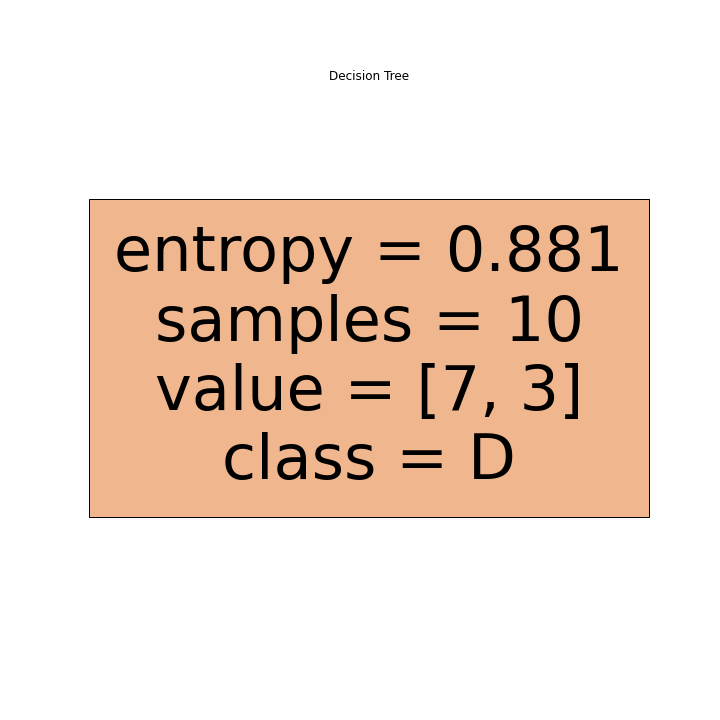
\includegraphics[width=0.5\linewidth]{tree_high.png}
			\caption{Decision Tree High}\label{tree high}
		\end{figure}
		
		\begin{figure}[h!]
			\centering
			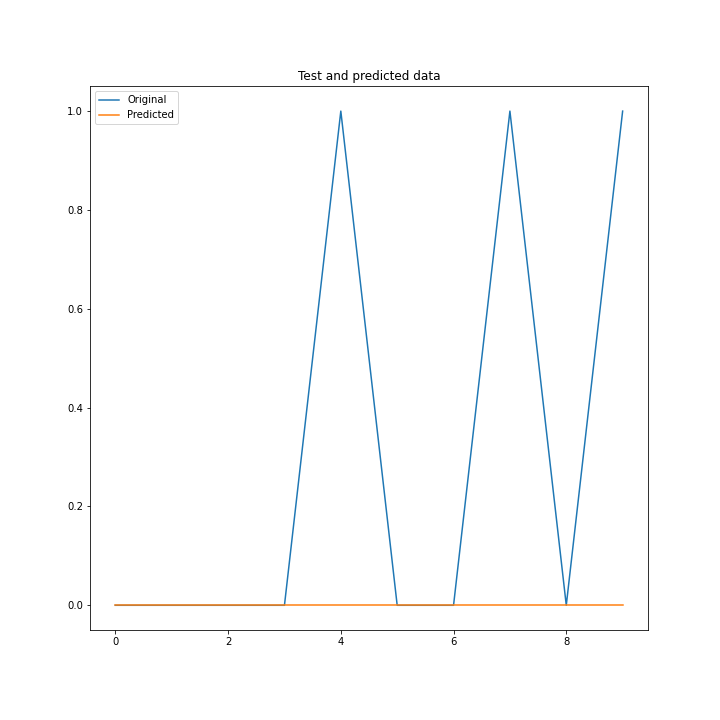
\includegraphics[width=0.5\linewidth]{tree_high_predition_vs_original.png}
			\caption{Predictions vs Originals High Tree}\label{tree pred high}
		\end{figure}
	
		\end{itemize}
	
	\pagebreak
	\item  Train another tree, but this time use a minimum impurity decrease of 0.1. Plot the resulting decision tree, and compare the results with the previous model you trained. Save the produced tree into ./output/tree\_low.png.
		\begin{itemize}
			\item I pre-process the data to one hot encode the categorical variables as the DecisionTreeClassifier does not work with strings. I then join back onto the dataframe to bring in the income. Using the default values except for Random State, IG as the splitter, and impurity decrease, I create a decision tree. We see with the minimum impurity decrease as 0.1, the decision tree gains additional branches. The generated model and tree is visible in \ref{tree low} and \ref{tree pred low}.  Ultimately, it classifies not married people with an annual income greater than 77.5 but less than 122.5 into the 'defaulter' class. and everyone else into the 'non-defaulter' class.
			
							
			\begin{figure}[h!]
				\centering
				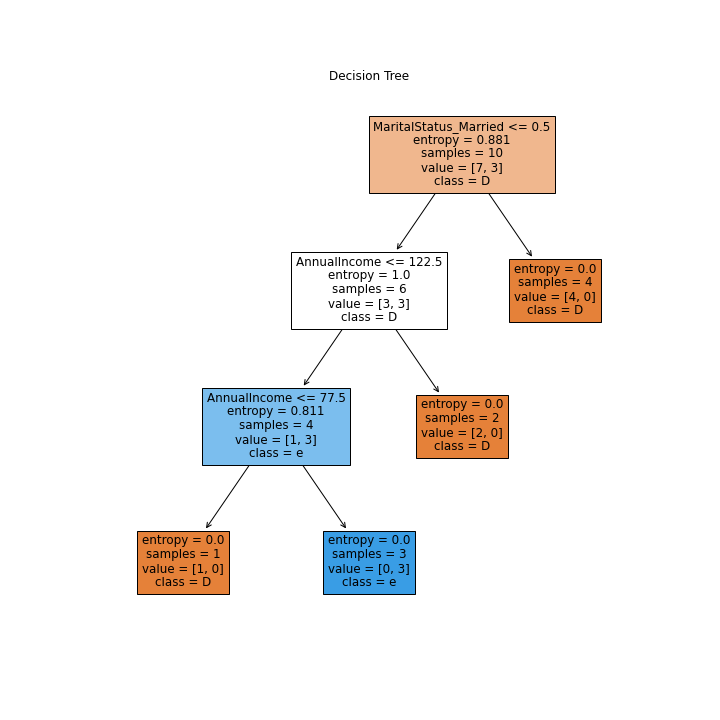
\includegraphics[width=0.5\linewidth]{tree_low.png}
				\caption{Decision Tree Low}\label{tree low}
			\end{figure}
			
			\begin{figure}[h!]
				\centering
				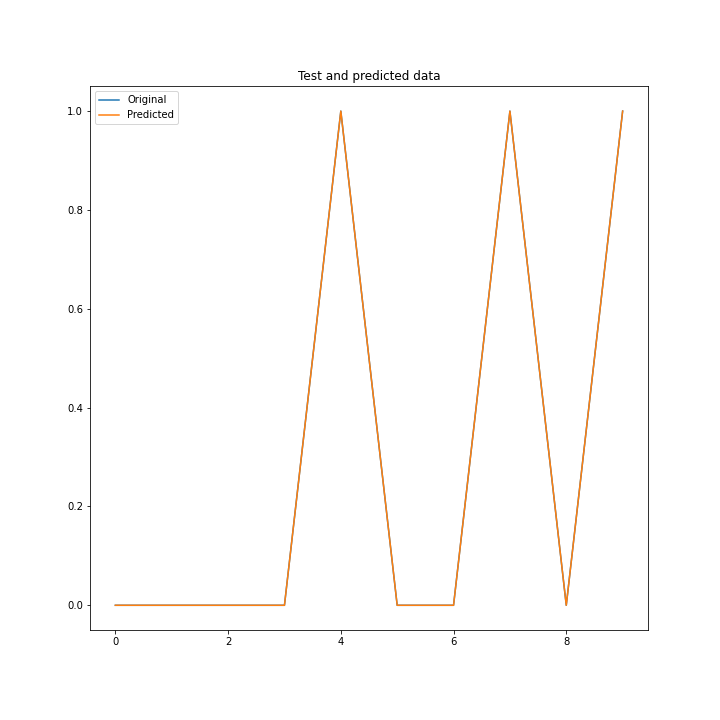
\includegraphics[width=0.5\linewidth]{tree_low_predition_vs_original.png}
				\caption{Predictions vs Originals High Tree}\label{tree pred low}
			\end{figure}
		\end{itemize}
	\pagebreak
	\item  Discuss the generated models in your report.
\begin{itemize}
	\item Please see discussion above. The low model classifies not married people with an annual income greater than 77.5 but less than 122.5 into the 'defaulter' class. and everyone else into the 'non-defaulter' class, while the high model classifies everyone into the non-defaulter class. Ultimately, the low model is superior, however we have a low volume of data.
	\item In both cases, the volume of data is far too low to make any proper comparison or insight into the model performance.
\end{itemize}

\item As a general note, throughout this assignment I have trained/tested/fit the model on the full dataset as the data volume is far too low for training or test splits. This is not a good practice and as such the performance claims need to be taken with caution.
\end{enumerate}
%
%	\item 
%\begin{itemize}
%	\item 
%\end{itemize}
%
%	\item 
%\begin{itemize}
%	\item 
%\end{itemize}
%
%	\item 
%\begin{itemize}
%	\item 
%\end{itemize}
%
%	\item 
%\begin{itemize}
%	\item 
%\end{itemize}	

\end{enumerate}
	
\end{document}
